
\begin{figure}
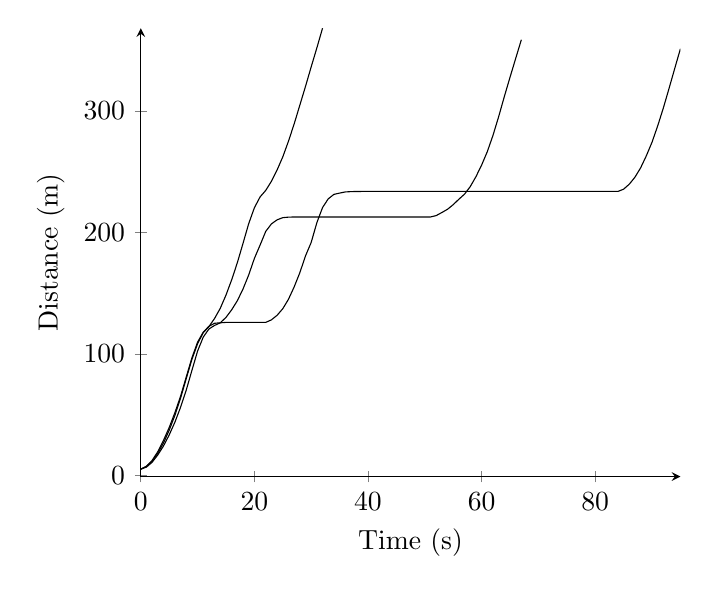
\begin{tikzpicture}
\begin{axis}[
legend style={anchor=west},
axis x line=bottom,
axis y line=left,
ymin=-1,
xlabel=Time (s),
ylabel=Distance (m),
]
\addplot[] coordinates {
(0, 5.1)
(1, 7.39431178683)
(2, 11.5845150261)
(3, 18.1856178451)
(4, 26.6200218299)
(5, 37.096784769)
(6, 49.2711495939)
(7, 63.4546346505)
(8, 79.5443684516)
(9, 95.432831772)
(10, 108.335158785)
(11, 117.458544439)
(12, 122.470082803)
(13, 129.198165887)
(14, 137.560057158)
(15, 148.386189779)
(16, 160.926668612)
(17, 175.049474763)
(18, 190.982119662)
(19, 207.205554815)
(20, 220.303675522)
(21, 229.184339564)
(22, 234.589790694)
(23, 242.097045331)
(24, 251.407035704)
(25, 262.188995263)
(26, 275.068513162)
(27, 289.260405688)
(28, 304.738748041)
(29, 320.226402945)
(30, 336.279655523)
(31, 351.942554183)
(32, 368.113725303)
};
\addplot[] coordinates {
(0, 5.1)
(1, 7.46434072634)
(2, 12.2936098998)
(3, 19.5059584808)
(4, 28.7819886538)
(5, 39.339628996)
(6, 51.4720520266)
(7, 65.0193393841)
(8, 80.8509812401)
(9, 96.6303253539)
(10, 109.666897175)
(11, 117.890315609)
(12, 122.706577137)
(13, 125.196475378)
(14, 125.588835371)
(15, 125.904302128)
(16, 125.937237174)
(17, 125.937237174)
(18, 125.937237174)
(19, 125.937237174)
(20, 125.937237174)
(21, 125.937237174)
(22, 125.937237174)
(23, 128.005739281)
(24, 131.756424129)
(25, 137.189900219)
(26, 144.955204079)
(27, 155.065626493)
(28, 166.813236785)
(29, 180.677460678)
(30, 191.717980779)
(31, 208.046773547)
(32, 220.452214268)
(33, 227.625403966)
(34, 231.315291238)
(35, 232.368361931)
(36, 233.311565125)
(37, 233.594159479)
(38, 233.70819922)
(39, 233.734545485)
(40, 233.734545485)
(41, 233.734545485)
(42, 233.734545485)
(43, 233.734545485)
(44, 233.734545485)
(45, 233.734545485)
(46, 233.734545485)
(47, 233.734545485)
(48, 233.734545485)
(49, 233.734545485)
(50, 233.734545485)
(51, 233.734545485)
(52, 233.734545485)
(53, 233.734545485)
(54, 233.734545485)
(55, 233.734545485)
(56, 233.734545485)
(57, 233.734545485)
(58, 233.734545485)
(59, 233.734545485)
(60, 233.734545485)
(61, 233.734545485)
(62, 233.734545485)
(63, 233.734545485)
(64, 233.734545485)
(65, 233.734545485)
(66, 233.734545485)
(67, 233.734545485)
(68, 233.734545485)
(69, 233.734545485)
(70, 233.734545485)
(71, 233.734545485)
(72, 233.734545485)
(73, 233.734545485)
(74, 233.734545485)
(75, 233.734545485)
(76, 233.734545485)
(77, 233.734545485)
(78, 233.734545485)
(79, 233.734545485)
(80, 233.734545485)
(81, 233.734545485)
(82, 233.734545485)
(83, 233.734545485)
(84, 233.734545485)
(85, 235.588886086)
(86, 239.726591381)
(87, 245.46878388)
(88, 253.210330764)
(89, 263.062533141)
(90, 274.241916612)
(91, 287.684909574)
(92, 302.507601464)
(93, 318.551190637)
(94, 334.953302581)
(95, 351.218689514)
};
\addplot[] coordinates {
(0, 5.1)
(1, 6.75050886513)
(2, 10.7623890263)
(3, 16.8077239972)
(4, 24.1564275469)
(5, 33.2047142838)
(6, 43.6541331259)
(7, 55.9465689872)
(8, 70.0870821729)
(9, 86.3298357387)
(10, 102.253302587)
(11, 113.837462694)
(12, 120.482578531)
(13, 123.442473677)
(14, 125.562372737)
(15, 130.042104693)
(16, 136.259824561)
(17, 143.764653949)
(18, 153.383722513)
(19, 164.967595275)
(20, 178.561328402)
(21, 189.510866316)
(22, 200.84164484)
(23, 206.992790209)
(24, 210.352017334)
(25, 212.155662432)
(26, 212.570825963)
(27, 212.704926305)
(28, 212.726629574)
(29, 212.726629574)
(30, 212.726629574)
(31, 212.726629574)
(32, 212.726629574)
(33, 212.726629574)
(34, 212.726629574)
(35, 212.726629574)
(36, 212.726629574)
(37, 212.726629574)
(38, 212.726629574)
(39, 212.726629574)
(40, 212.726629574)
(41, 212.726629574)
(42, 212.726629574)
(43, 212.726629574)
(44, 212.726629574)
(45, 212.726629574)
(46, 212.726629574)
(47, 212.726629574)
(48, 212.726629574)
(49, 212.726629574)
(50, 212.726629574)
(51, 212.726629574)
(52, 213.838095363)
(53, 216.36688587)
(54, 219.047473374)
(55, 222.84266066)
(56, 227.330931923)
(57, 231.523551761)
(58, 237.697836993)
(59, 245.845409421)
(60, 255.381699211)
(61, 266.435893336)
(62, 279.826215285)
(63, 295.236701919)
(64, 311.796717259)
(65, 327.6876149)
(66, 343.213471451)
(67, 358.647534533)
};

\end{axis}
\end{tikzpicture}
\label{tik:0:16_O, 17_S, 17_S.-60, 19_V}
\caption{0 percent diving with GSC on route $16_O, 17_S, 17_S.-60, 19_V$}
\end{figure}
